\documentclass[letterpaper,landscape]{article}

\usepackage[margin=20mm]{geometry}
\usepackage{tikz}
\usepackage{graphicx}

\begin{document}
\thispagestyle{empty}
\begin{center}

{\Large\textbf{Print at EXACTLY 100\% scale. Do not "Fit to Page".}}\\
\vspace{2mm}
Cut along the outer black boundary (187.5\,mm\,$\times$\,142.0\,mm) and tape to the platform.

\vspace{5mm}

\begin{tikzpicture}[x=1mm, y=1mm]

  % 1. Outer platform boundary: exactly 187.5 mm wide, 142.0 mm high.
  \draw[thick] (0, 0) rectangle (187.5, -142.0);

  % 2. Six ArUco markers, each rendered 22.5 mm wide.
  %    The inner black square is 15 mm (67% of 22.5 mm = white border stripped).
  %    Centres are inset 12 mm from each edge.

  % Top-Left   (ID 0)  -- physical (12, 12)
  \node at (12, -12)    {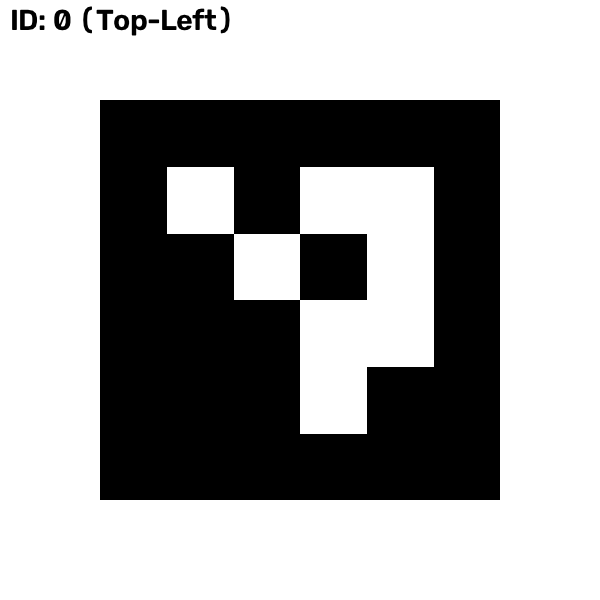
\includegraphics[width=22.5mm]{aruco/marker_0.png}};
  % Top-Right  (ID 1)  -- physical (175.5, 12)
  \node at (175.5, -12)   {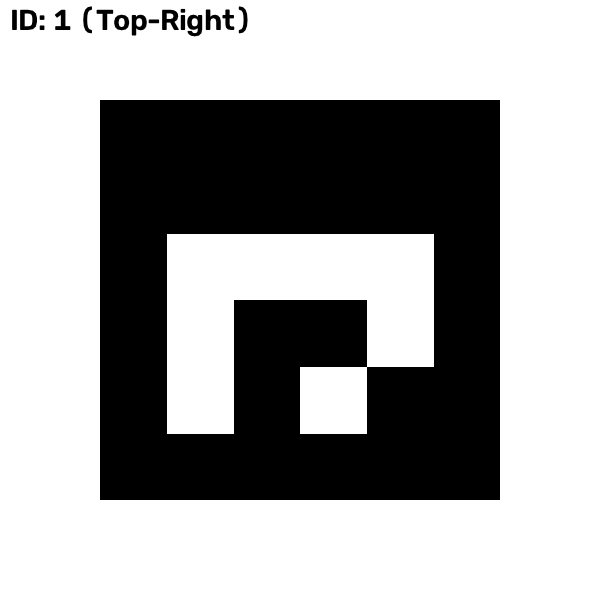
\includegraphics[width=22.5mm]{aruco/marker_1.png}};
  % Bottom-Right (ID 2) -- physical (175.5, 130)
  \node at (175.5, -130)  {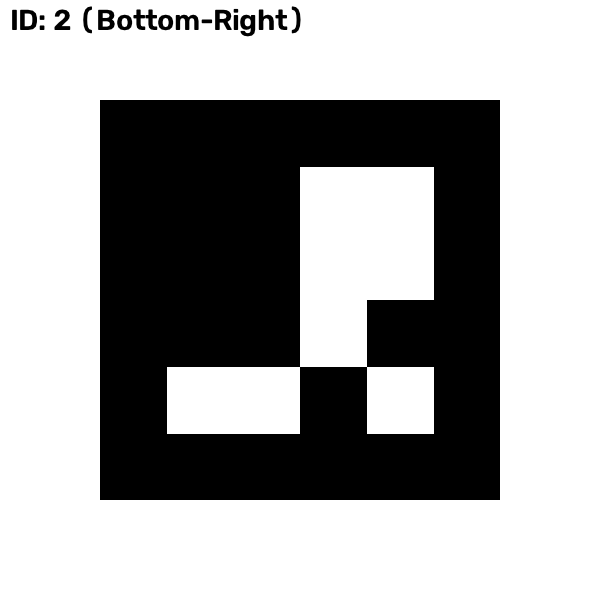
\includegraphics[width=22.5mm]{aruco/marker_2.png}};
  % Bottom-Left  (ID 3) -- physical (12, 130)
  \node at (12, -130)   {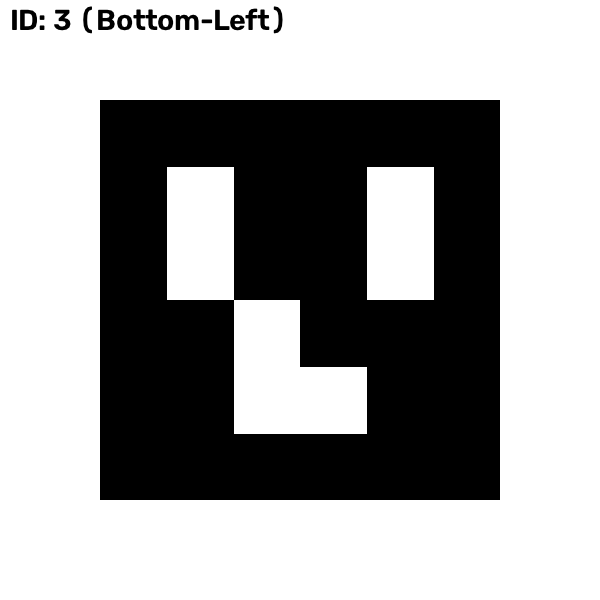
\includegraphics[width=22.5mm]{aruco/marker_3.png}};
  % Middle-Left  (ID 4) -- physical (12, 71)
  \node at (12, -71)    {
\includegraphics[width=22.5mm]{aruco/marker_4.png}};
  % Middle-Right (ID 5) -- physical (175.5, 71)
  \node at (175.5, -71)   {
\includegraphics[width=22.5mm]{aruco/marker_5.png}};

  % 3. Centre crosshair for visual reference only.
  \draw[gray, dashed] (93.75, -71) circle (5mm);
  \draw[gray, dashed] (83.75, -71) -- (103.75, -71);
  \draw[gray, dashed] (93.75, -61) -- (93.75, -81);

\end{tikzpicture}
\end{center}
\end{document}
